\documentclass[11pt]{article}
\usepackage[utf8]{inputenc}
%\geometry{showframe}% for debugging purposes -- displays the margins

%% ys
\usepackage[shortlabels]{enumitem}
\usepackage{geometry}
\usepackage{bm}
\usepackage{amssymb}
\usepackage{algorithm}
\usepackage{algpseudocode}
\usepackage{xcolor}
\usepackage{algorithm, algorithmic} % for algorithms
\usepackage{listings}
\geometry{a4paper,scale=0.75}
\newcommand{\jie}{$\star$ }
\newcommand{\by}{\bm{y}}
\newcommand{\bx}{\bm{x}}
\newcommand{\iid}{\overset{\text{iid}}{\sim}}
\newcommand{\half}{\frac{1}{2}}
\newcommand{\ynote}[1]{\color{red} #1 \color{black}}
%% ys

%\geometry{showframe}% for debugging purposes -- displays the margins

\newcommand{\E}{\mbox{E}}

\usepackage{amsmath}
%\usepackage[garamond]{mathdesign}
\usepackage{url}

% Set up the images/graphics package
\usepackage{graphicx}
\setkeys{Gin}{width=\linewidth,totalheight=\textheight,keepaspectratio}
\graphicspath{{graphics/}}

\title{Exercises 2: Generalized linear models}
%\author[ ]{ }
\date{}  % if the \date{} command is left out, the current date will be used

% The following package mwakes prettier tables.  We're all about the bling!
\usepackage{booktabs}

% The units package provides nice, non-stacked fractions and better spacing
% for units.
\usepackage{units}

% The fancyvrb package lets us customize the formatting of verbatim
% environments.  We use a slightly smaller font.
\usepackage{fancyvrb}
\fvset{fontsize=\normalsize}

% Small sections of multiple columns
\usepackage{multicol}

% Provides paragraphs of dummy text
\usepackage{lipsum}

% These commands are used to pretty-print LaTeX commands
\newcommand{\doccmd}[1]{\texttt{\textbackslash#1}}% command name -- adds backslash automatically
\newcommand{\docopt}[1]{\ensuremath{\langle}\textrm{\textit{#1}}\ensuremath{\rangle}}% optional command argument
\newcommand{\docarg}[1]{\textrm{\textit{#1}}}% (required) command argument
\newenvironment{docspec}{\begin{quote}\noindent}{\end{quote}}% command specification environment
\newcommand{\docenv}[1]{\textsf{#1}}% environment name
\newcommand{\docpkg}[1]{\texttt{#1}}% package name
\newcommand{\doccls}[1]{\texttt{#1}}% document class name
\newcommand{\docclsopt}[1]{\texttt{#1}}% document class option name

\newcommand{\N}{\mbox{N}}
\newcommand{\thetahat}{\hat{\theta}}
\newcommand{\sigmahat}{\hat{\sigma}}
\newcommand{\betahat}{\hat{\beta}}


\begin{document}

\maketitle% this prints the handout title, author, and date

\section{Exponential families}

We say that a distribution $f(y; \theta, \phi)$ is in an exponential family if we can write its PDF or PMF in the form
$$
f(y; \theta, \phi) = \exp \left\{ \frac{y \theta - b(\theta)}{a(\phi)} + c(y; \phi)   \right \}
$$
for some known functions $a$, $b$ and $c$.  We refer to $\theta$ as the canonical parameter of the family, and  (for reasons that will become clear) to $\phi$ as the dispersion parameter.  

\begin{enumerate}[(A)]

\item Starting from the ``standard'' form of each PDF/PMF, show that the following distributions are in an exponential family, and find the corresponding $b$, $c$, $\theta$, and $a(\phi)$.  

\begin{itemize}
\item $Y \sim N(\mu, \sigma^2)$ for known $\sigma^2$.  
\item $Y = Z/N$ where $Z \sim \mbox{Binom}(N, P)$ for known $N$.   
\item $Y \sim \mbox{Poisson}(\lambda)$  
\end{itemize}

\bigskip
\jie
\begin{enumerate}
    \item 
    \begin{align*}
    p(y) &= (2\pi\sigma^2)^{-\half} \exp \{ -\frac{1}{2\sigma^2} (y-\mu)^2 \} \\
    &= \exp \{ -\frac{y^2}{2\sigma^2} + \frac{2y\mu}{2\sigma^2} -\frac{\mu^2}{2\sigma^2} - \half \log (2\pi\sigma^2) \} \\
    &= \exp \{ \frac{y\mu -\half \mu^2}{\sigma^2} + [-\frac{y^2}{2\sigma^2} - \half \log (2\pi\sigma^2)] \}
\end{align*}
Therefore,
\begin{align*}
    \theta &= \mu \\
    b(\mu) &= \half \mu^2 \\
    \phi &= \sigma^2 \\
    c(y;\sigma^2) &= -\frac{y^2}{2\sigma^2} - \half \log (2\pi\sigma^2) \\
    a(\sigma^2) &= \sigma^2
\end{align*}
    
    \item 
    We have $z = yN$,
    \begin{align*}
        p(z) &= N {N \choose z} P^z (1-P)^{N-z} \\
        p(y) &= N {N \choose yN} P^{yN} (1-P)^{N-yN} \cdot N \\
        &= \exp\{ \log\left[N{N \choose yN}\right] + yN \log P + (1-y)N\log (1-P) \} \\
        &= \exp \{y[N\log P - N \log (1-P)] + N \log (1-P) + \log\left[N{N \choose yN}\right]\} \\
        &= \exp \{\frac{y \log \frac{P}{1-P}}{1/N} + N \log (1-P) + \log\left[N{N \choose yN}\right]\}
    \end{align*}
    Let $\theta = \log \frac{P}{1-P}$, then $P = \frac{e^\theta}{1+e^\theta}$ and $1-P = \frac{1}{1+e^\theta}$,
    \begin{align*}
        p(z) &= \exp \{\frac{y \log \frac{P}{1-P}}{1/N} + N \log (1-P) + \log\left[N{N \choose yN}\right]\} \\
        &= \exp \{\frac{y \theta}{1/N} - N \log (1+e^\theta) + \log\left[N{N \choose yN}\right]\} \\
        &= \exp \{\frac{y \theta - \log (1+e^\theta)}{1/N} + \log\left[N{N \choose yN}\right]\}
    \end{align*}
    Therefore,
    \begin{align*}
    \theta &= \log \frac{P}{1-P} \\
    b(\theta) &= \log (1+e^\theta) \\
    \phi &= N \\
    c(y;N) &= \log\left[N{N \choose yN}\right] \\
    a(N) &= \frac{1}{N}
    \end{align*}
    
    \item 
    \begin{align*}
        p(y) &= \frac{\lambda^y e^{-\lambda}}{y!} \\
        &= \exp \{ y\log \lambda - \lambda -\log(y!) \}
    \end{align*}
    Let $\theta = \log \lambda$,
    \begin{align*}
        p(y) &= \exp \{ y\theta - e^\theta - \log(y!)\}
    \end{align*}
    Therefore,
    \begin{align*}
    \theta &= \log  \lambda \\
    b(\theta) &= e^\theta \\
    c(y;\phi) &= - \log(y!) \\
    a(\phi) &= 1
    \end{align*}
    
\end{enumerate}
\bigskip

\item We want to characterize the mean and variance of a distribution in the exponential family.  To do this, we'll take an unfamiliar route, involving a preliminary lemma (that holds much more generally than just the exponential family).  Define the \emph{score} $s(\theta)$ as the gradient of the log likelihood with respect to the parameter of interest:  
$$
s(\theta) = \frac{\partial}{\partial \theta} \log L(\theta) \, , \quad L(\theta) = \sum_{i=1}^n f(y_i; \theta) \, .
$$
\ynote{A typo? }
We've written this in multivariate form for the sake of generality, but of course it just involves an ordinary partial derivative (w.r.t.~$\theta$) in the case where $\theta$ is one-dimensional.
%Let's also define $H(\theta)$ as the Hessian matrix, i.e.~the matrix of second partial derivatives of the log likelihood:
%$$
%H(\theta) = \frac{\partial}{\partial \theta^T} s(\theta) =   \frac{\partial^2}{ \partial \theta \partial \theta^T} \log L(\theta)
%$$

While we think of the score as a function of $\theta$, clearly (just like the likelihood) the score also depends on the data.  So a natural question is: what can we say about the \emph{distribution} of the score over different random realizations of the data under the true data-generating process, i.e.~at the true $\theta$?  It turns out we can say the following, sometimes referred to as the score equations:  
$$
\begin{aligned}
E\{ s(\theta) \} &= 0 \\
\mathcal{I}(\theta) \equiv \mbox{var} \{ s(\theta) \}  &= - E \left\{ H(\theta) \right\}
\end{aligned}
$$
where the mean and variance are taken under the true $\theta$.  \textbf{Prove the score equations.}  Hints: prove the first equation first.  You can assume that it's OK to switch the order of differentiation and integration (i.e.~that any necessary technical conditions are met).  To prove the second equation, differentiate both sides of the first equation with respect to $\theta^T$ and switch the order of differentiation and integration again.  Expand out and simplify.  

\bigskip
\jie
\begin{align*}
    E\{s(\theta)\} &= E\{ \frac{\partial}{\partial \theta} \sum_{i=1}^n \log f(y_i;\theta) \} \\
    &= E\{ \sum_{i=1}^n \frac{\frac{\partial}{\partial \theta}f(y_i;\theta)}{f(y_i;\theta)} \} \\
    &= \sum_{i=1}^n E\{\frac{\frac{\partial}{\partial \theta}f(y_i;\theta)}{f(y_i;\theta)} \} \\
    &= \sum_{i=1}^n \int \frac{\frac{\partial}{\partial \theta}f(y_i;\theta)}{f(y_i;\theta)} f(y_i;\theta) dy_i\\
    &= \sum_{i=1}^n \int \frac{\partial}{\partial \theta}f(y_i;\theta) dy_i \\
    &= \sum_{i=1}^n \frac{\partial}{\partial \theta} \int f(y_i;\theta) dy_i
\end{align*}
Because $\int f(y_i;\theta) dy_i  = 1, \; \forall i$, 
$$\frac{\partial}{\partial \theta} \int f(y_i;\theta) dy_i = 0.$$
Therefore,
$$E\{s(\theta)\} = 0.$$

Denote $f(y;\theta) = \prod_{i=1}^n f(y_i,\theta)$.
\begin{align*}
    0 &= \frac{\partial}{\partial \theta^T} E\{s(\theta)\} \\
    &= \frac{\partial}{\partial \theta^T} E\{\frac{\partial}{\partial \theta} \log f(y;\theta) \} \\
    &= \frac{\partial}{\partial \theta^T} \int \frac{\partial}{\partial \theta} \log f(y;\theta) \cdot f(y;\theta)dy \\
    &= \int \frac{\partial}{\partial \theta^T} \left[ \frac{\partial}{\partial \theta} \log f(y;\theta) \cdot f(y;\theta) \right]dy \\
    &= \int \frac{\partial^2}{\partial \theta \partial \theta^T} \log f(y;\theta) \cdot f(y;\theta) + \frac{\partial}{\partial \theta} \log f(y;\theta) \cdot \frac{\partial}{\partial \theta^T} f(y;\theta) dy \\
    &= \int \frac{\partial^2}{\partial \theta \partial \theta^T} \log f(y;\theta) \cdot f(y;\theta) + \frac{\partial}{\partial \theta} \log f(y;\theta) \cdot \left[\frac{\partial}{\partial \theta}  f(y;\theta) \right]^T dy \\
    &= E\{\frac{\partial^2}{\partial \theta \partial \theta^T} \log f(y;\theta)\} + \int \frac{\partial}{\partial \theta} \log f(y;\theta) \cdot \left[\frac{\partial}{\partial \theta}  f(y;\theta) \right]^T dy \\
    &= E\{\frac{\partial^2}{\partial \theta \partial \theta^T} \log f(y;\theta)\} + \int \frac{\partial}{\partial \theta} \log f(y;\theta) \cdot \left[\frac{\partial}{\partial \theta}  \log f(y;\theta) \cdot f(y;\theta) \right]^T dy \\
    &= E\{\frac{\partial^2}{\partial \theta \partial \theta^T} \log f(y;\theta)\} + \int \frac{\partial}{\partial \theta} \log f(y;\theta) \cdot \left[\frac{\partial}{\partial \theta}  \log f(y;\theta) \right]^T  \cdot f(y;\theta) dy \\
    &= E\{\frac{\partial^2}{\partial \theta \partial \theta^T} \log f(y;\theta)\} + E\{s(\theta)s(\theta)^T\}
\end{align*}
Then,
\begin{align*}
    Var\{s(\theta)\} &= E\{s(\theta)s(\theta)^T\} - E\{s(\theta)\}E\{s(\theta)\}^T \\
    &= E\{s(\theta)s(\theta)^T\} \\
    &= - E\{\frac{\partial^2}{\partial \theta \partial \theta^T} \log f(y;\theta)\} \\
    &= -E\{H(\theta)\}
\end{align*}
\bigskip

\item Use the score equations you just proved to show that, if $Y \sim f(y; \theta, \phi)$ is in an exponential family, then
$$
\begin{aligned}
E(Y) &=  b'(\theta) \\
\mbox{var} ( Y ) &= a(\phi) b''(\theta) 
\end{aligned}
$$

Thus the variance of $Y$ is a product of two terms.  One of these terms, $b''(\theta)$, depends only on the canonical parameter $\theta$, and hence on the mean, since you showed that $E(Y) =  b'(\theta)$.  The other, $a(\phi)$, is independent of $\theta$.  Note that the most common form of $a$ is $a(\phi) = \phi/w$, where $\phi$ is called a dispersion parameter and where $w$ is a known prior weight that can vary from one observation to another; we'll see this below.  

\bigskip
\jie
The pdf is
$$
f(y; \theta, \phi) = \exp \left\{ \frac{y \theta - b(\theta)}{a(\phi)} + c(y; \phi)   \right \}
$$
The expectation is
$$
E(Y) = \int y \exp \left\{ \frac{y \theta - b(\theta)}{a(\phi)} + c(y; \phi)   \right \} dy
$$
Because
$$ \int \exp \left\{ \frac{y \theta - b(\theta)}{a(\phi)} + c(y; \phi)   \right \} dy = 1,$$
\begin{align*}
    0 &= \frac{\partial}{\partial \theta} \int \exp \left\{ \frac{y \theta - b(\theta)}{a(\phi)} + c(y; \phi)   \right \} dy \\
    &= \int \frac{\partial}{\partial \theta}  \exp \left\{ \frac{y \theta - b(\theta)}{a(\phi)} + c(y; \phi)   \right \} dy \\
    &= \int \frac{y - b'(\theta)}{a(\phi)}  \exp \left\{ \frac{y \theta - b(\theta)}{a(\phi)} + c(y; \phi)   \right \} dy \\
    &= E(Y) - b'(\theta)
\end{align*}
Therefore,
$$E(Y) = b'(\theta).$$

Because
$$0 = \int \frac{y - b'(\theta)}{a(\phi)}  \exp \left\{ \frac{y \theta - b(\theta)}{a(\phi)} + c(y; \phi)   \right \} dy,$$
\begin{align*}
    0 &= \frac{\partial}{\partial \theta} \int \frac{y - b'(\theta)}{a(\phi)}  \exp \left\{ \frac{y \theta - b(\theta)}{a(\phi)} + c(y; \phi)   \right \} dy \\
    &= \int \frac{\partial}{\partial \theta} \frac{y - b'(\theta)}{a(\phi)}  \exp \left\{ \frac{y \theta - b(\theta)}{a(\phi)} + c(y; \phi)   \right \} dy\\
    &= \int -b''(\theta)  \exp \left\{ \frac{y \theta - b(\theta)}{a(\phi)} + c(y; \phi)   \right \} + \left[ \frac{y - b'(\theta)}{a(\phi)} \right]^2  \exp \left\{ \frac{y \theta - b(\theta)}{a(\phi)} + c(y; \phi)   \right \} dy \\
    &= -\frac{b''(\theta)}{a(\phi)} + \frac{1}{a(\phi)^2} \{ E(Y^2) -  2b'(\theta)E(Y) + b'(\theta)^2 \} \\
    &= -\frac{b''(\theta)}{a(\phi)} + \frac{1}{a(\phi)^2} \{ E(Y^2) -  [E(Y)]^2 \} \\
    &= -\frac{b''(\theta)}{a(\phi)} + \frac{Var(Y)}{a(\phi)^2}
\end{align*}
Therefore,
$$Var(Y) = a(\phi)b''(\theta).$$

\item To convince yourself that your result in $(C)$ is correct, use these results to compute the mean and variance of the $N(\mu, \sigma^2)$ distribution.  

\bigskip
\jie
$Y \sim N(\mu,\sigma^2)$, we have
\begin{align*}
    \theta &= \mu \\
    b(\mu) &= \half \mu^2 \\
    \phi &= \sigma^2 \\
    c(y;\sigma^2) &= -\frac{y^2}{2\sigma^2} - \half \log (2\pi\sigma^2) \\
    a(\sigma^2) &= \sigma^2
\end{align*}
Then, mean
\begin{align*}
    E(Y) &= b'(\theta) =\mu,
\end{align*}
and variance
$$Var(Y) = a(\phi)b''(\theta) = \sigma^2 \cdot 1 = \sigma^2.$$

\end{enumerate}


\section{Generalized linear models}  

Suppose we observe data like in the typical regression setting: that is, pairs $\{y_i, x_i\}$ where $y_i$ is a scalar response for case $i$, and $x_i$ is a $p$-vector of predictors or features for that same case $i$.  We say that the $y_i$'s follow a \textit{generalized linear model} (GLM) if two conditions are met.  First, the PDF (or PMF, if discrete) can be written as:  
$$
f(y_i; \theta_i,  \phi)  = \exp \left\{ \frac{y_i \theta_i - b(\theta_i)}{\phi/w_i} + c(y_i; \phi/w_i)   \right \}
$$
where the weights $w_i$ are all known.  This is referred to as the stochastic or random component of the model.  Second, for some known invertible function $g$ we have
$$
g(\mu_i) = x_i^T \beta
$$
where $\mu_i = E(Y_i; \theta_i, \phi)$.  This is the systematic component of the model, and $g$ is referred to as a link function, since it links the mean of the response $\mu_i$ with the \emph{linear predictor} $\eta_i = x_i^T \beta$.  


\begin{enumerate}[(A)]

\item Deduce from your results above that, in a GLM,
 $$
\begin{aligned}
\theta_i &= (b')^{-1} \Big( g^{-1}(x_i^T \beta) \Big) \\
\mbox{var} (Y_i ) &= \frac{\phi}{w_i} V(\mu_i)
\end{aligned}
$$
for some function $V$ that you should specify in terms of the building blocks of the exponential family model.  $V$ is often referred to as a the \emph{variance function}, since it explicitly relates the mean and the variance in a GLM.  

\bigskip
\jie
From the results above, $E(Y_i) = b'(\theta)$. Because $g(\mu_i) = x_i^T\beta$,
$$\mu_i = E(Y_i) = b'(\theta_i) = g^{-1}(x_i^T\beta).$$
Therefore,
$$\theta_i = (b')^{-1} \Big( g^{-1}(x_i^T \beta) \Big).$$
\begin{align*}
    Var(Y_i) &= a(\phi)b''(\theta) \\
    &= \frac{\phi}{w_i} b''( (b')^{-1} \mu_i)
\end{align*}

\bigskip

\item Take two special cases.  
\begin{enumerate}[(1)]
\item Suppose that $Y$ is a Poisson GLM, i.e. that the stochastic component of the model is a Poisson distribution.  Show that $V(\mu) = \mu$.
\item Suppose that $Y = Z/N$ is a Binomial GLM, i.e. that the stochastic component of the model is a Binomial distribution $Z \sim \mbox{Binom}(N, P)$ and that $Y$ is the fraction of yes outcomes (1's).  Show that $V(\mu) = \mu(1-\mu)$.  
\end{enumerate}

\bigskip
\begin{enumerate}
    \item For Poisson distribution, $b(\theta) = e^\theta$
\begin{align*}
    V(\mu) &= b''( (b')^{-1} \mu)\\
    &=b''(\log \mu) \\
    &= \exp\{\log \mu\} \\
    &= \mu
\end{align*}

    \item $b(\theta) = \log(1+e^\theta)$, $b'(\theta) = \frac{e^\theta}{1+e^\theta}$, $b''(\theta) = \frac{e^\theta}{(1+e^\theta)^2}$
\begin{align*}
    V(\mu) &= b''( (b')^{-1} \mu)\\
    &=b''(\log \frac{\mu}{1-\mu}) \\
    &= \frac{\frac{\mu}{1-\mu}}{(1+\frac{\mu}{1-\mu})^2} \\
    &= \mu(1-\mu)
\end{align*}

\end{enumerate}




\item To specify a GLM we must choose the link function $g(\mu_i)$.  Recall that $g$ links the predictors with the mean of the response: $g(\mu_i) = x_i^T \beta$.  Since you've shown that
$$
\theta_i = (b')^{-1} \left\{g^{-1}(x_i^T \beta) \right\} \, ,
$$
a ``simple'' choice of link function is one where $g^{-1} = b'$, or equivalently $g(\mu) = (b')^{-1}(\mu)$.  This is known as the \textit{canonical link}, in which case the canonical parameter simplifies to
$$
\theta_i = (b')^{-1} \left\{b'(x_i^T \beta) \right\} = x_i^T \beta \, .
$$
So under the canonical link $g(\mu) = b'^{-1}(\mu)$, we have the model
$$
f(y_i; \beta, \phi) \exp \left\{ \frac{y_i x_i^T \beta - b(x_i^T \beta)}{\phi/w_i} + c(y_i; \phi/w_i)   \right \}
$$

Now return to the two special cases from the previous problem.
\begin{enumerate}[(1)]
\item Suppose that $Y$ is a Poisson GLM, i.e. that the stochastic component of the model is a Poisson distribution. Show that the canonical link is the log link, $g(\mu) = \log \mu$.  
\item Suppose that $Y = Z/N$ is a Binomial GLM, i.e. that the stochastic component of the model is a Binomial distribution $Z \sim \mbox{Binom}(N, P)$.   Show that the canonical link is the logistic link $g(\mu) = \log \left\{ \mu/(1-\mu) \right\}$.  
\end{enumerate}

\bigskip
\jie
Poisson. $b(\theta) = e^\theta$, then
$$g(\mu) = b'(\mu) = \log \mu.$$

Binomial. $b(\theta) = \log(1+e^\theta)$, then
$$g(\mu) = b'(\mu) = \log \left\{ \mu/(1-\mu) \right\}.$$

\end{enumerate}



\section{Fitting GLMs}

 The regression coefficients $\beta$ in a GLM are typically fit using some variation on likelihood-based inference.  To this end, define the likelihood function for a given GLM as
$$
L(\beta, \phi) = \prod_{i=1}^n \exp \left\{ \frac{y_i \theta_i - b(\theta_i)}{\phi/w_i} + c(y_i; \phi/w_i)   \right \} \, ,
$$
where based on results you proved above, we define $\theta_i = (b')^{-1}(\mu_i)$ and $\mu_i = g^{-1}(x_i^T \beta)$.  This allows us to define the score function $s(\beta, \phi)$ as the gradient of the log likelihood with respect to $\beta$:
$$
s(\beta, \phi) = \nabla_\beta \  \log L(\beta, \phi) = \frac{\partial}{\partial \beta} \log L(\beta, \phi) \, .
$$



\begin{enumerate}[(A)]

\item Using the chain rule
$$
\frac{\partial}{\partial \beta} = \frac{\partial}{\partial \theta} \times \frac{\partial \theta}{\partial \mu } \times \frac{\partial \mu}{\partial \beta} \, ,
$$
show that 
$$
s(\beta, \phi) \equiv \nabla_\beta \  \log L(\beta, \phi)  = \sum_{i=1}^n \frac{w_i(Y_i - \mu_i) x_i}{ \phi V(\mu_i) g'(\mu_i)}
$$
where $x_i$ is the vector of predictors for case $i$ (i.e.~row $i$ of the predictor matrix $X$, transposed to be a column vector). 

\bigskip
\jie
\begin{align*}
    s(\beta, \phi) &= \nabla_\beta \  \log L(\beta, \phi) = \frac{\partial}{\partial \beta^T} \log L(\beta, \phi) \\
    &= \frac{\partial}{\partial \theta} \left\{ \sum_{i=1}^n \frac{y_i \theta_i - b(\theta_i)}{\phi/w_i} + c(y_i; \phi/w_i) \right\} \frac{\partial \theta}{\partial \mu} \frac{\partial \mu}{\partial \beta}
\end{align*}
$$\frac{\partial}{\partial \theta} \left\{ \sum_{i=1}^n \frac{y_i \theta_i - b(\theta_i)}{\phi/w_i} + c(y_i; \phi/w_i) \right\} = \left(\dots, \frac{y_i-b'(\theta_i)}{\phi/w_i},\dots \right).$$
Because $\theta_i = (b')^{-1} (\mu_i)$, 
$$\frac{\partial \theta_i}{\partial \mu_i} = \frac{1}{b''((b')^{-1}\mu_i)} = \frac{1}{V(\mu_i)}.$$
Then,
$$\frac{\partial \theta}{\partial \mu} = \text{diag}\left(\dots,\frac{1}{V(\mu_i)},\dots\right).$$
Because $\mu_i = g^{-1}(x_i^T\beta)$,
$$\frac{\partial \mu_i}{\partial \beta} = \frac{x_i^T}{g'(g^{-1}(x_i^T\beta))} = \frac{x_i^T}{g'(\mu_i)}.$$
Then,
\begin{align*}
    \frac{\partial \mu}{\partial \beta} =  
    \begin{bmatrix}
      & \dots & \\
    \dots & \frac{x_i^T}{g'(\mu_i)} & \dots \\
      & \dots &
    \end{bmatrix}
\end{align*}
Therefore,
\begin{align*}
    \frac{\partial}{\partial \beta} \log L(\beta, \phi) &= \frac{\partial}{\partial \theta} \left\{ \sum_{i=1}^n \frac{y_i \theta_i - b(\theta_i)}{\phi/w_i} + c(y_i; \phi/w_i) \right\} \frac{\partial \theta}{\partial \mu} \frac{\partial \mu}{\partial \beta} \\
    &= \begin{bmatrix}
      \dots & \frac{y_i-b'(\theta_i)}{\phi/w_i} & \dots
    \end{bmatrix}
    \begin{bmatrix}
      \ddots & & \\
      & \frac{1}{V(\mu_i)} & \\
      & & \ddots
    \end{bmatrix}
    \begin{bmatrix}
      & \dots & \\
    \dots & \frac{x_i^T}{g'(\mu_i)} & \dots \\
      & \dots &
    \end{bmatrix} \\
    &= 
    \begin{bmatrix}
     \dots & \frac{(y_i-b'(\theta_i))w_i}{\phi V(\mu_i)} & \dots
    \end{bmatrix}
    \begin{bmatrix}
      & \dots & \\
    \dots & \frac{x_i^T}{g'(\mu_i)} & \dots \\
      & \dots &
    \end{bmatrix} \\
    &= \sum_{i=1}^n \frac{w_i(y_i - \mu_i) x_i^T}{ \phi V(\mu_i) g'(\mu_i)}
\end{align*}
Therefore,
$$s(\beta, \phi) = \sum_{i=1}^n \frac{w_i(y_i - \mu_i) x_i}{ \phi V(\mu_i) g'(\mu_i)}.$$
\bigskip

\item Show that under the canonical link, $g'(\mu) = 1/V(\mu)$, so that the score function simplifies to:  
$$
s(\beta, \phi) = \sum_{i=1}^n \frac{w_i(Y_i - \mu_i) x_i}{ \phi} \, .
$$

Hint: remember from calculus that
$$
(g^{-1})'(x) = \frac{1}{g'\left\{ g^{-1}(x) \right\}}
$$
\bigskip
\jie 
Under the canonical link, i.e., $g(\mu) = (b')^{-1}(\mu)$, 
$$g'(\mu) = (b'^{-1})'(\mu) = \frac{1}{b''((b')^{-1}(\mu))} = \frac{1}{V(\mu)}. $$
When $g'(\mu) = 1/V(\mu)$,
\begin{align*}
    s(\beta, \phi) &= \sum_{i=1}^n \frac{w_i(y_i - \mu_i) x_i}{ \phi V(\mu_i) g'(\mu_i)} \\
    &= \sum_{i=1}^n \frac{w_i(Y_i - \mu_i) x_i}{ \phi}
\end{align*}

\item Let's take the specific case of a GLM for a binomial outcome, where $Y_i \sim \mbox{Binom}(N_i, \mu_i)$ for known sample size $N_i$, $Y_i = Z_i/N_i$ is the observed success fraction, and where $\mu_i$ is related to the predictors $x_i \in \mathcal{R}^p$ via the (canonical) logistic link.  This is called the logistic regression model.  But how should we fit the parameters?

Read up on the method of steepest descent, i.e.~gradient descent\footnote{if you want a textbook reference, see \textit{Numerical optimization}, by Nocedal and Wright. This should be available in electronic form through from the UT Library website.}  Write your own function that will fit a logistic regression model by gradient descent.  For extra coding brownie points, try to maintain some level of generality to your code, i.e. so that it could also work with different GLMs, assuming your wrote different sub-routines.  

Grab the data ``wdbc.csv'' from the course website, or obtain some other real data that interests you, and test out your fitter.  The WDBC file has information on 569 breast-cancer patients from a study done in Wisconsin.  The first column is a patient ID, the second column is a classification of a breast cell (Malignant or Benign), and the next 30 columns are measurements computed from a digitized image of the cell nucleus.  These are things like radius, smoothness, etc.  For this problem, use the first 10 features for $X$, i.e.~columns 3-12 of the file.  (If you use all 30 features you'll run into trouble.) 

Some notes:
\begin{itemize}
\item We're trying to maximize the log likelihood function, but the convention in the optimization literature is to minimize things.  No big deal; what we're doing is the same as \textit{minimizing} the negative of the log likelihood.  
\item You need to add an intercept term, and the simplest way is to add a column of 1's as the first column of the feature matrix $X$.  (If you've never seen this trick before, convince yourself why it makes sense.)  
\item Make sure that, at every iteration of gradient descent, you compute and store the current value of the log likelihood, so that you can track and plot the convergence of the algorithm.
\item Be sensitive to the numerical consequences of an estimated success probability that is either very near 0, or very near 1.
\item Finally, you can be as clever as you want about the gradient-descent step size.  Small step sizes will be more robust but slower; larger step sizes can be faster but may overshoot and diverge; step sizes based on line search (Chapter 3 of Nocedal and Wright) are cool but involve some extra, optional work.
\end{itemize}

\bigskip
\jie
The GLM for binomial outcome, $V(\mu) = \mu(1-\mu)$, $b(\theta) = \log(1+e^\theta)$.
Under the canonical link, $g(\mu) = \log \frac{\mu}{1-\mu}$.
We have $$f(y) = \exp \{\frac{y \theta - \log (1+e^\theta)}{1/N} + \log\left[N{N \choose yN}\right]\},$$
therefore, in 
$$
L(\beta, \phi) = \prod_{i=1}^n \exp \left\{ \frac{y_i \theta_i - b(\theta_i)}{\phi/w_i} + c(y_i; \phi/w_i)   \right \} \, ,
$$
$$\phi = 1; \; w_i = N_i.$$
Therefore, the score function under the canonical link is
\begin{align*}
    s(\beta, \phi) &= \nabla_\beta \  \log L(\beta, \phi) \\
    &= \sum_{i=1}^n \frac{w_i(Y_i - \mu_i) x_i}{ \phi} \\
    & = \sum_{i=1}^n N_i (Y_i - \mu_i) x_i \\
    &= \sum_{i=1}^n N_i \left(Y_i - \frac{\exp(x_i^T\beta)}{1+\exp(x_i^T\beta)} \right) x_i
\end{align*}

Using the gradient descent,
$$ \beta \leftarrow \beta + \gamma s(\beta, \phi),$$
where $\gamma$ is the step size.

Determinate the step size by line search.
\begin{algorithm}
\begin{algorithmic}
\caption{Gradient descent for GLM}
\Require Starting value $\beta^0$
\While{not converge}
    \State $\gamma \leftarrow \arg \max_\gamma logL(\beta^{m-1} + \gamma s(\beta^{m-1}, \phi))$ (Line search) 
    \State $ \beta^{m} \leftarrow \beta^{m-1} + \gamma s(\beta^{m-1}, \phi)$
    \If{$\left|\frac{logL(\beta^{m}) - logL(\beta^{m-1})}{logL(\beta^{m-1})} \right| < tol$}
    \State Converge
    \EndIf
\EndWhile
\end{algorithmic}
\end{algorithm}

\begin{figure}[h]
    \centering
    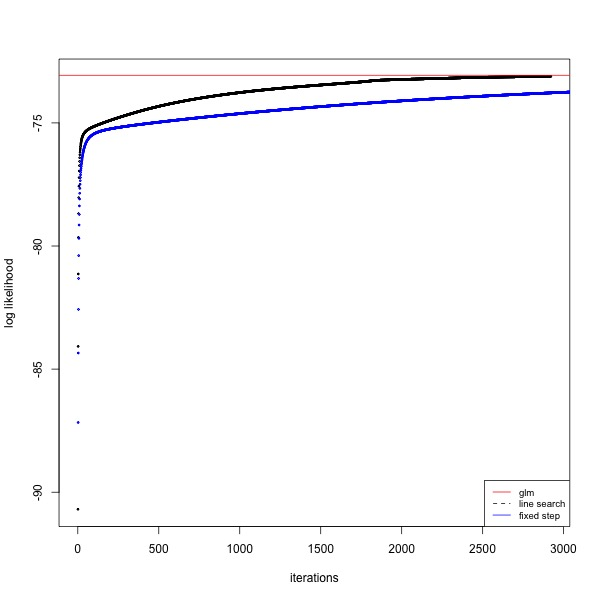
\includegraphics[width=0.7\textwidth]{figures/logl.jpg}
    \caption{The log likelihood over the iterations}
    \label{fig:logl_GD}
    \end{figure}


\item Consider the Hessian matrix, i.e. the matrix of partial second derivatives of the log likelihood:  
$$
H(\beta, \phi) = \frac{\partial^2}{\partial \beta \partial \beta^T} \log L(\beta, \phi) 
$$
Give an expression for the Hessian matrix $H(\beta, \phi)$ of a GLM that is as simple as possible, ideally in matrix form.   Note: to keep things a little more streamlined, please assume the canonical link function here; it's the same idea, just with hairier algebra, under an arbitrary link function.  

\bigskip
\jie
From the previous question, we have
$$ \log L(\beta) = \sum_{i=1}^n \frac{y_i \theta_i - b(\theta_i)}{\phi/w_i} + c(y_i; \phi/w_i).$$
$$ \nabla_\beta \  \log L(\beta, \phi)  = \frac{\partial}{\partial \beta^T} \log L(\beta, \phi) = \sum_{i=1}^n \frac{w_i(y_i - \mu_i) x_i}{ \phi V(\mu_i) g'(\mu_i)}$$
The Hessian matrix is
\begin{align*}
    H(\beta, \phi) &= \frac{\partial^2}{\partial \beta \partial \beta^T} \log L(\beta, \phi) \\
    &= \frac{\partial}{\partial \beta} \left\{ \sum_{i=1}^n \frac{w_i(y_i - \mu_i) x_i}{ \phi V(\mu_i) g'(\mu_i)} \right\} \\
    &= \frac{\partial}{\partial \mu} \left\{ \sum_{i=1}^n \frac{w_i(y_i - \mu_i) x_i}{ \phi V(\mu_i) g'(\mu_i)} \right\} \frac{\mu}{\partial \beta} \\
    &= 
    \begin{bmatrix}
      \dots & -\frac{w_ix_i}{\phi} & \dots
    \end{bmatrix}
    \begin{bmatrix}
      \vdots \\
      \frac{x_i^T}{g'(\mu_i)} \\
      \vdots
    \end{bmatrix} \\
    & = - \sum_{i=1}^n \frac{w_i x_i x_i^T}{\phi g'(\mu_i)}
\end{align*}
The $(k,j)$th element in $H(\beta, \phi)$ is
$$H_{k,j}(\beta, \phi) = - \sum_{i=1}^n \frac{w_ix_{ki}x_{ij}}{\phi g'(\mu_i)} .$$
Therefore,
$$H(\beta,\phi) = - X^T W X,$$
where $X$ is the feature matrix and 
$$W = diag \left(\dots, \frac{w_i}{\phi g'(\mu_i)}, \dots \right).$$

\item Now consider a point $\beta_0 \in \mathcal{R}^P$, which serves as an intermediate guess for our vector of regression coefficients.  Show that, for any GLM, the second-order Taylor approximation of $\log L(\beta, \phi)$, around the point $\beta_0$, can be expressed in the form
$$
q(\beta; \beta_0) = -\frac{1}{2}(\tilde{y} - X \beta)^T W (\tilde{y} - X \beta) + c\, ,
$$
where $\tilde{y}$ is a vector of ``working responses'' and $W$ is a diagonal matrix of ``working weights,'' and $c$ is a constant that doesn't involve $\beta$.  Give explicit expressions for the diagonal elements $W_{ii}$ and for $\tilde{y}$ (which will necessarily involve the point $\beta_0$, around which you're doing the expansion).\footnote{Remember the trick of completing the square, e.g.~\url{https://davidrosenberg.github.io/mlcourse/Notes/completing-the-square.pdf}.} Again, we're assuming the canonical link to make the algebra a bit simpler.  

\bigskip
\jie
The second order Taylor approximation
\begin{align*}
    q(\beta;\beta_0) &= \log L(\beta_0) + \nabla_\beta \log L(\beta)^T|_{\beta= \beta_0} \cdot (\beta - \beta_0) + \half (\beta - \beta_0)^T H(\beta_0) (\beta - \beta_0)
\end{align*}
Let $W = W|_{\beta = \beta_0}$, which means $W$ is a diagonal matrix and 
$$W_{ii} = \frac{w_i}{\phi g'(\mu_{i0})},$$
where $\mu_{i0} = \mu_i|_{\beta= \beta_0} = g^{-1}(x_i^T\beta_0)$. 
Then
\begin{align*}
    q(\beta;\beta_0) &= \log L(\beta_0) + \nabla_\beta \log L(\beta)^T|_{\beta= \beta_0} \cdot (\beta - \beta_0) + \half (\beta - \beta_0)^T X^T W X (\beta - \beta_0)
\end{align*}
The gradient
\begin{align*}
    \nabla_\beta \log L(\beta)^T &= \sum_{i=1}^n \frac{w_i(y_i - \mu_i) x_i^T}{ \phi} \\
    &=  \sum_{i=1}^n (y_i - \mu_i)g'(\mu_i) \frac{w_i }{ \phi g'(\mu_i)} x_i^T \\
    &= 
    \begin{bmatrix}
      \dots & (y_i - \mu_i)g'(\mu_i) & \dots
    \end{bmatrix}
    WX
\end{align*}
Then, the second term in $q(\beta;\beta_0)$ is 
\begin{align*}
    \text{2nd term} &= \begin{bmatrix}
      \dots & (y_i - \mu_{i0})g'(\mu_{i0}) & \dots
    \end{bmatrix}
    WX (\beta - \beta_0) \\
    &= \tilde{z}^T W X (\beta- \beta_0)
\end{align*}
where $\tilde{z} = \begin{bmatrix}
      \dots & (y_i - \mu_{i0})g'(\mu_{i0}) & \dots
    \end{bmatrix}$, $\mu_{i0} = \mu_i|_{\beta= \beta_0} = g^{-1}(x_i^T\beta_0)$. 
Therefore, 
\begin{align*}
    q(\beta;\beta_0) &= \log L(\beta_0) + \nabla_\beta \log L(\beta)^T|_{\beta= \beta_0} \cdot (\beta - \beta_0) + \half (\beta - \beta_0)^T H(\beta_0) (\beta - \beta_0) \\
    &=  \log L(\beta_0) + \tilde{z}^T W X (\beta- \beta_0) - \half (\beta - \beta_0)^T X^T W X (\beta - \beta_0) \\
    &= -\half \beta^T X^T W X \beta  + \beta_0^T X^T W X \beta + \tilde{z}^T W X \beta + \tilde{c} \\
    &= -\half \beta^T X^T W X \beta + (\tilde{z}^T + \beta_0^T X^T) W X\beta + \tilde{c} \\
    &= -\half \beta^T X^T W X \beta + \tilde{y}^T W X \beta + \tilde{c} \\
    &= -\frac{1}{2}(\tilde{y} - X \beta)^T W (\tilde{y} - X \beta) + c
\end{align*}
where 
\begin{align*}
    \tilde{y}^T = 
    \begin{bmatrix}
      \dots &  (y_i - \mu_{i0})g'(\mu_{i0}) + x_i^T \beta_0 & \dots
    \end{bmatrix}
\end{align*}


\item  Read up on Newton's method for optimizing smooth functions (e.g. in Nocedal and Wright, Chapter 2).  Implement it for the logistic regression model model and test it out on the same data set you just used to test out gradient descent.\footnote{Hey, cool!  You should be able to use your own solver for weighted least squares that you wrote for the first set of problems.}  Note: while you could do line search, there is a ``natural'' step size of 1 in Newton's method.  Verify that your solution replicates the $\beta$ estimate you get when using a package solver, e.g. the glm function in R, up to minor numerical differences.  

\bigskip
\jie
The newton method is as follows
\begin{algorithm}[H]
\begin{algorithmic}
\caption{Newton method for GLM}
\Require Starting value $\beta^0$
\While{not converge}
    \State $ \beta^{m} \leftarrow \beta^{m-1} - H^{-1} \nabla_\beta\log L$
    \If{$\left|\frac{logL(\beta^{m}) - logL(\beta^{m-1})}{logL(\beta^{m-1})} \right| < tol$}
    \State Converge
    \EndIf
\EndWhile
\end{algorithmic}
\end{algorithm}
The Hessian
$$H(\beta,\phi) = - X^T W X,$$
where $X$ is the feature matrix and 
$$W = diag \left(\dots, \frac{w_i}{\phi g'(\mu_i)}, \dots \right).$$
$$\frac{w_i}{\phi g'(\mu_i)} = \frac{1}{g'(\mu_i)} = \mu_i(1-\mu_i).$$

\begin{figure}[h]
    \centering
    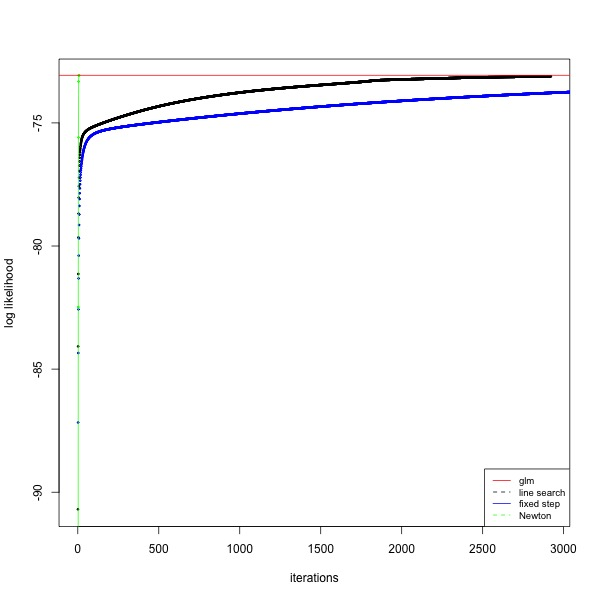
\includegraphics[width=0.7\textwidth]{figures/logl_2.jpg}
    \caption{The log likelihood over the iterations}
    \label{fig:logl_Newton}
    \end{figure}
    
Figure \ref{fig:logl_Newton} shows the log likehood. Newton method converges after 8 iterations and the estimated $\beta$ is very close to the estimation in function glm().

\begin{lstlisting}[language=R]
> beta_glm - beta
             [,1]
     4.453896e-08
V3  -6.427526e-07
V4   3.235037e-08
V5   2.255286e-07
V6   5.692142e-07
V7   2.297304e-08
V8  -2.619810e-10
V9   2.998861e-09
V10  4.171561e-08
V11  1.139896e-08
V12 -1.706985e-08
\end{lstlisting}

\bigskip

\item Standard asymptotic theory, which we won't go into here, implies that the maximum likelihood estimator is consistent and asymptotically normal around the true value $\beta_0$:
$$
\hat{\beta} \sim N(\beta_0, I(\beta_0, \phi)^{-1}) \, ,
$$
where $\mathcal{I}(\beta_0, \phi)$, called the \textit{Fisher information matrix}, is the same $\mathcal{I}$ you met all the way back when you proved the score equations:  
$$
\mathcal{I}(\beta_0, \phi) \equiv \mbox{var} \{ s(\beta_0, \phi) \}  = - E \left\{ H(\beta_0, \phi) \right\} \, .
$$
The fact that Fisher information is the negative of the expected Hessian motivates the following idea: use the inverse of the negative Hessian matrix at the MLE to approximate the inverse Fisher information, i.e.~the covariance matrix of the estimator.  Happily, you get this Hessian matrix for free when fitting by Newton's method.

For your logistic regression on the WDBC data fit via Newton's method, compute the square root of each diagonal element of the inverse Hessian matrix, evaluated at the MLE.\footnote{These are your standard errors for each coefficient, i.e.~the square root of the variance of each coefficient's (approximate) sampling distribution.}  Compare these to the standard errors you get when using a package solver, e.g. the glm function in R.  

The square root of each diagonal element of the inverse Hessian matrix is very close to the standard errors using the glm function in R.  
\begin{lstlisting}[language=R]
> # sqrt of diag of inverse negative Hessian
> sqrt(diag(solve(-H)))
                   V3         V4         V5         V6         V7         V8         V9        V10        V11 
 0.5642741 13.0939632  0.2775461 12.2742249  5.8903905  0.4493906  1.0742854  0.6473007  1.1069398  0.2914167 
       V12 
 0.6040244 
> std_glm <- summary(fit)$coefficients[,2]
> # std error in glm()
> std_glm
(Intercept)          V3          V4          V5          V6          V7          V8          V9         V10 
  0.5643200  13.0949439   0.2775752  12.2749905   5.8909033   0.4494181   1.0743433   0.6473276   1.1070102 
        V11         V12 
  0.2914299   0.6040610 
\end{lstlisting}


\end{enumerate}


\end{document}

